% Define document class & import showyourwork
\documentclass[twocolumn]{aastex631}

% Begin!
\begin{document}

% Title
\title{An open source scientific article}

% Author list
\author{@rodluger}

% Abstract
\begin{abstract}
    This is a sample open source scientific article automatically generated using the \texttt{showyourwork} package.
    The icons in the right margin of the abstract link to the \texttt{GitHub} repository containing the source code and to the build logs for the workflow that generated this PDF on \texttt{GitHub Actions}.
\end{abstract}

% Main body
\section{Introduction}
This article was automatically generated from a repository containing a TeX file,
a \texttt{conda} environment file, some \texttt{Python} figure scripts, and a \texttt{Snakefile} with custom instructions for downloading external datasets.
Edit the TeX file, figure scripts, and \texttt{Snakefile} as needed, and whenever you commit and push your changes to \texttt{GitHub}, this PDF will automatically regenerate on \texttt{GitHub Actions}. Please check out the \texttt{showyourwork} \href{https://github.com/rodluger/showyourwork}{repository} for more information.

% A sample two-panel figure
\begin{figure}[ht!]
    \begin{centering}
        \includegraphics[width=0.4\linewidth]{mandelbrot.pdf}
        \includegraphics[width=0.4\linewidth]{koch.pdf}
        \caption{
            A sample plot with two subpanels.
            Both figures were generated from the same \texttt{Python} script in the \texttt{figures} directory.
            The name of the script is inferred from the figure label in the TeX file.
        }
        % This label tells showyourwork that the script `figures/fractals.py'
        % generates the two PDF files included above
        \label{fig:fractals}
    \end{centering}
\end{figure}

% A sample figure generated from an external dataset
\begin{figure}[ht!]
    \begin{centering}
        \includegraphics[width=0.4\linewidth]{fibonacci.pdf}
        \caption{
            Another sample plot.
            This one was generated from a dataset hosted on Zenodo; the instructions for downloading this dataset are specified in the \texttt{Snakefile}.
        }
        % This label tells showyourwork that the script `figures/fibonacci.py'
        % generates the PDF included above
        \label{fig:fibonacci}
    \end{centering}
\end{figure}

% A static figure, committed directly to the repository
% https://en.wikipedia.org/wiki/File:Romanesco_broccoli_(Brassica_oleracea).jpg
% Creative Commons Attribution-Share Alike 4.0 International License
% https://creativecommons.org/licenses/by-sa/4.0/deed.en
\begin{figure}[ht!]
    \begin{centering}
        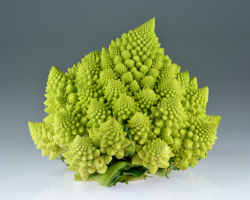
\includegraphics[width=0.4\linewidth]{broccoli.pdf}
        \caption{
            A sample figure that was directly committed to the repository.
            Committing output isn't generally recommended, but for certain figure types (like photographs or flowcharts), it makes sense.
        }
        % The asterisk below tells showyourwork not to look for a script
        % that generates this figure, and that the PDF already exists
        \label{fig*:broccoli}
    \end{centering}
\end{figure}

Here is an inline figure that's not part of a \verb+figure+ environment: \includegraphics[width=1em]{inline.pdf}. Since \texttt{showyourwork} can't automatically infer the script that generated it, a custom rule must be included in the \texttt{Snakefile} to produce it.

\end{document}
